
\section{Asynchronous Monitoring}

%-------------------------------------------------------------------------
\begin{frame}{Asynchronous Monitoring}



\note{each local monitor obtains a partial view (i.e., a concrete local state) of the system's global state. It communicates with other monitors through a shared memory and updates its knowledge, and then solely based on its partial view, emits a final verdict. We show how, given any \LTL formula and an \Exltl, a set of verdicts collectively provided by the local monitors can be used to compute the verdict computed by a centralized monitor that has full view of the system under scrutiny.}


\begin{block}{Asynchronous Monitoring}

The system under inspection produces a finite trace $\alpha = \state_0 \state_1 \cdots \state_k$, and is inspected with respect to an \LTL formula $\varphi$ by a set $\monitor = \{ M_1, M_2, \cdots , M_n \}$ of asynchronous distributed monitors.

\end{block}


\begin{block}{Local Monitor Algorithm}

\begin{figure}
 \centering
 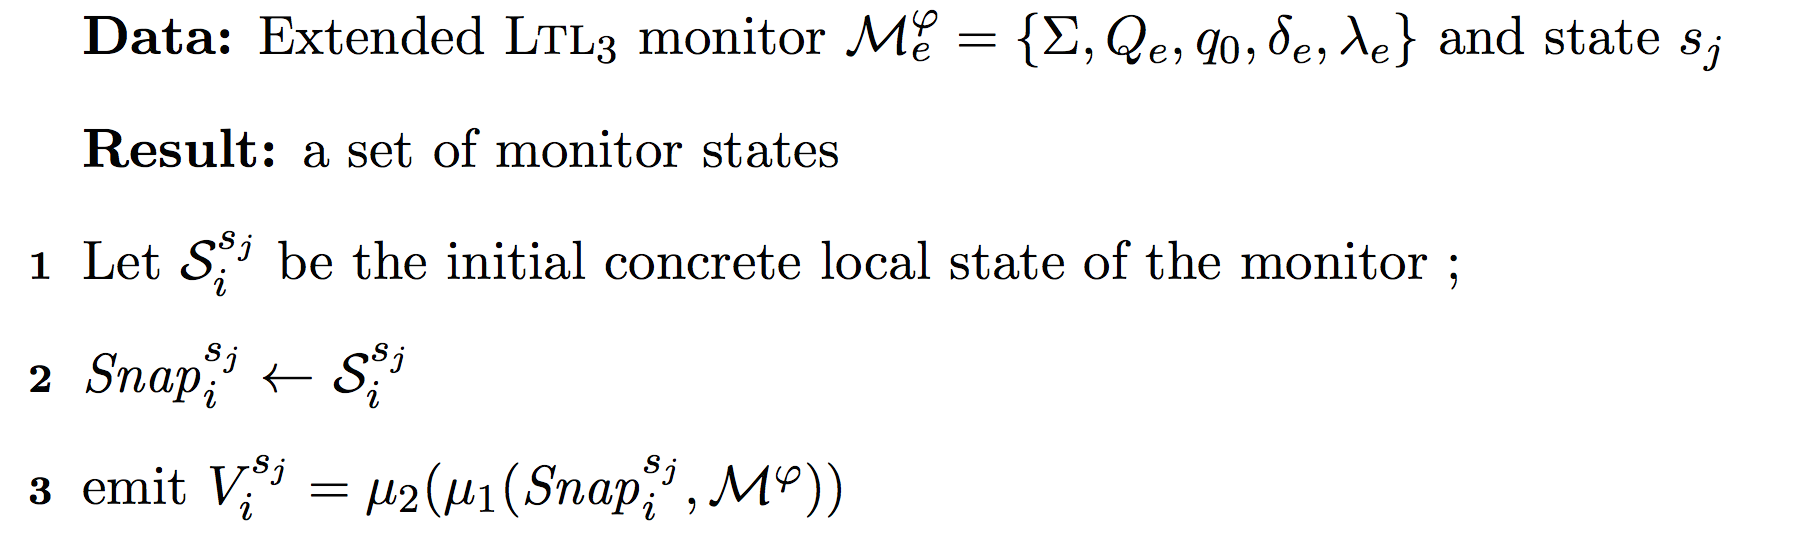
\includegraphics[scale=.25, angle=-360]{figures/asynchalgo}
 \end{figure}


\end{block}

\end{frame}



\begin{frame}{Asynchronous Monitoring}


\begin{example}

 Let $\varphi = \F (a \wedge b)$ whose \Exltl~is given below. Suppose monitors are at monitor state $\monstate_0$, and let $\state= \{a, b\} $ be the global state of the system. \\

\ \\

\begin{figure}[H]
\centering
\begin{tikzpicture}[->,>=stealth',shorten >=1pt,auto,node distance=4.8cm,
                    semithick, initial text={}, initial where=right]
  \tikzstyle{every state}=[scale=0.55, every node/.style={scale=0.65}]

  \node[initial,state] (A)                {$\monstate_0$};
  \node[state, accepting]         (B) [left of  = A] {$\monstate_\top$};
  \node[state]         (D) [below of = B] {$\monstate_1$};

  \path (A) edge              node {$ \{a,b\}$} (B)
                 edge [loop above] node {$\{b\}, \emptyset$} (A)
                 edge      [bend left=20]     node   {$\{a\}$} (D)
        (B) edge [loop above] node {$\tru$} (B)
        (D) edge                 node {$\{a,b\}$} (B)
        (D) edge       [bend left=15]             node {$\{b\}, \emptyset$} (A)
        (D) edge [loop below] node {$\{a\}$} (D);

\end{tikzpicture}    

\end{figure}

\end{example}

\end{frame}



\begin{frame}

\begin{example}
The following tables represent each monitor $M_i$'s initial \localreg~$\snap_i^\state$ and its verdict set $\verdict_i$ calculated based on only $\snap_i^\state$.

\ \\


\begin{center}

 \begin{tabular}{|c|c|c|c|}
   \multicolumn{1}{r}{} &  \multicolumn{2}{c}{ {$\snap_1^\state$}}\\
\hline
  & $M_1$ & $M_2$ & $M_3$\\
 \hline
   $a$ & $\tru$ & $\udef$ & $\udef$\\
   $b$ & $\udef$ & $\udef$ & $\udef$\\
\hline
  $\verdict_1$  &  \multicolumn{3}{c|}{\cellcolor{gray!25}$\{\monstate_1, \monstate_\top\}$}\\
\hline
  \end{tabular}  
\quad
 \begin{tabular}{|c|c|c|c|}
   \multicolumn{1}{r}{} &  \multicolumn{2}{c}{ {$\snap_2^\state$}}\\
\hline
  & $M_1$ & $M_2$ & $M_3$\\
 \hline
   $a$ & $\udef$ & $\udef$ & $\udef$\\
   $b$ & $\udef$ & $\tru$ & $\udef$\\
\hline
  $\verdict_2$  &  \multicolumn{3}{c|}{\cellcolor{gray!25}$\{\monstate_0, \monstate_\top\}$}\\
\hline
  \end{tabular} 
%\quad

\end{center}


\begin{center}
 \begin{tabular}{|c|c|c|c|}
   \multicolumn{1}{r}{} &  \multicolumn{2}{c}{ {$\snap_3^\state$}}\\
\hline
  & $M_1$ & $M_2$ & $M_3$\\
 \hline
   $a$ & $\udef$ & $\udef$ & $\udef$\\
   $b$ & $\udef$ & $\udef$ & $\udef$\\
\hline
  $\verdict_3$  &  \multicolumn{3}{c|}{\cellcolor{gray!25}$\{\monstate_0, \monstate_1, \monstate_\top\}$}\\
\hline
  \end{tabular}   
\end{center}


$\verdict_1 \cap \verdict_2 \cap \verdict_3 = q_\top$.

\end{example}

\end{frame}








